% "Станет проще"

\documentclass[a4paper,12pt]{article} % тип документа

% report, book

% Рисунки
\usepackage{graphicx}
\usepackage{wrapfig}
\usepackage{hyperref}
\usepackage[rgb]{xcolor}
\pagestyle{plain}



%  Русский язык

\usepackage[T2A]{fontenc}			% кодировка
\usepackage[utf8]{inputenc}			% кодировка исходного текста
\usepackage[english,russian]{babel}	% локализация и переносы


% Математика
\usepackage{amsmath,amsfonts,amssymb,amsthm,mathtools} 


\usepackage{wasysym}

%Заговолок
\author{Сафиуллин Роберт	}
\title{Лабораторная работа 3.6.1\\ СПЕКТРАЛЬНЫЙ АНАЛИЗ ЭЛЕКТРИЧЕСКИХ СИГНАЛОВ}





\begin{document} % начало документа

\maketitle


\newpage
\section{Цель работы:}
исследование кривых намагничивания ферромагнетиков с помощью баллистического гальванометра.
\\
\section{В работе используются:}
генератор тока, блок питания, тороид, соленоид, баллистический гальванометр с осветителем и шкалой, амперметры, магазин сопротивлений, ЛАТР, разделительный трансформатор.

 
\section{Экспериментальная установка:}

 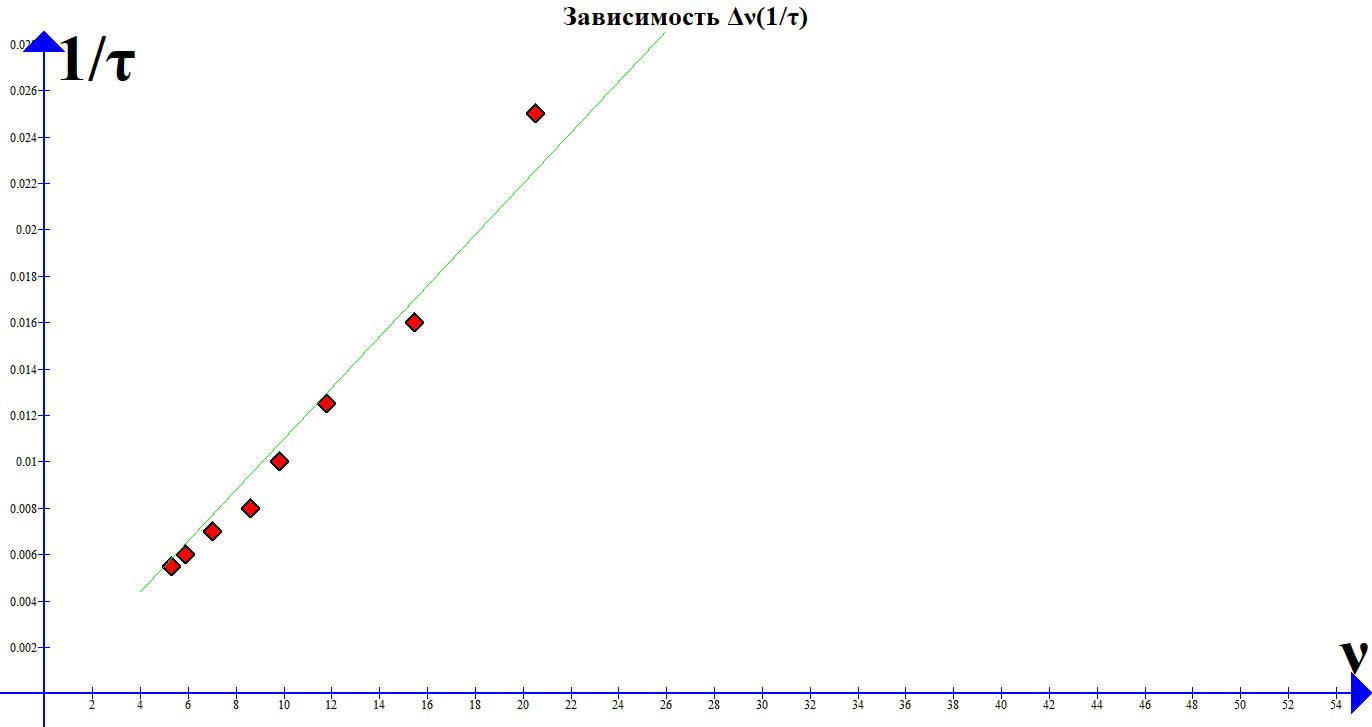
\includegraphics[scale=0.4]{3611}
\section{Ход работы}
1) СОбрали схему
2) Установили сопротивление 80 $\Omega$ и прошли по всей петле.
3) Убедившись, что зайчик нигде не выходит за шкалу, снимем показания:\\
\begin{tabular}{|c|c|}
\hline 
I, mA & $\Delta$x \\ 
\hline 
1470 & 0 \\ 
\hline 
530 & 12 \\ 
\hline 
244 & 12 \\ 
\hline 
147 & 8.6 \\ 
\hline 
96 & 6.6 \\ 
\hline 
65 & 5.1 \\ 
\hline 
50 & 3 \\ 
\hline 
40 & 2 \\ 
\hline 
34 & 1,2 \\ 
\hline 
31 & 0,7 \\ 
\hline 
27 & 1 \\ 
\hline 
23 & 0.9 \\ 
\hline 
0.6 & 7.2 \\ 
\hline 
0,00032 & 0.1 \\ 
\hline 
\end{tabular} 
Участок EFC'
\begin{tabular}{|c|c|}
\hline 
I, mA & $\Delta$x \\ 
\hline 
0.00032 & 0.1 \\ 
\hline 
0.6 & 12 \\ 
\hline 
23 & 2.9 \\ 
\hline 
27 & 4.1 \\ 
\hline 
31 & 4.6 \\ 
\hline 
34 & 13.6 \\ 
\hline 
40 & 23 \\ 
\hline 
50 & 22 \\ 
\hline 
65 & 21.5 \\ 
\hline 
96 & 16.6 \\ 
\hline 
147 & 15.6 \\ 
\hline 
244 & 19.2 \\ 
\hline 
540 & 15.4 \\ 
\hline 
1470 & 0 \\ 
\hline 
\end{tabular} 
C'E'
\begin{tabular}{|c|c|}
\hline 
I, mA & $\Delta$x \\ 
\hline 
1470 & 0 \\ 
\hline 
530 & 12.2 \\ 
\hline 
244 & 12.4 \\ 
\hline 
147 & 9 \\ 
\hline 
96 & 6.7 \\ 
\hline 
65 & 5.1 \\ 
\hline 
50 & 3 \\ 
\hline 
40 & 2 \\ 
\hline 
34 & 1.2 \\ 
\hline 
31 & 0.6 \\ 
\hline 
27 & 1 \\ 
\hline 
23 & 0.9 \\ 
\hline 
0.6 & 7.4 \\ 
\hline 
0,00032 & 0.1 \\ 
\hline 
E'C
\begin{tabular}{|c|c|}
\hline 
I, mA & $\Delta$x \\ 
\hline 
0.00032 & 0.1 \\ 
\hline 
0.6 & 12 \\ 
\hline 
23 & 2.9 \\ 
\hline 
27 & 4.1 \\ 
\hline 
31 & 4.6 \\ 
\hline 
34 & 13.6 \\ 
\hline 
40 & 23 \\ 
\hline 
50 & 22 \\ 
\hline 
65 & 21.5 \\ 
\hline 
96 & 16.6 \\ 
\hline 
147 & 15.6 \\ 
\hline 
244 & 19.2 \\ 
\hline 
540 & 15.4 \\ 
\hline 
1470 & 0 \\ 
\hline 
\end{tabular} 
\end{tabular} 


 

































\textbf{I Исследование спектра периодической последовательности прямоугольных импульсов}\\
1) Проанализируем как меняетсяя спектр при изменении параметров $\Delta$$\nu$ и $f_{povt}$
\begin{flushleft}
\begin{center}

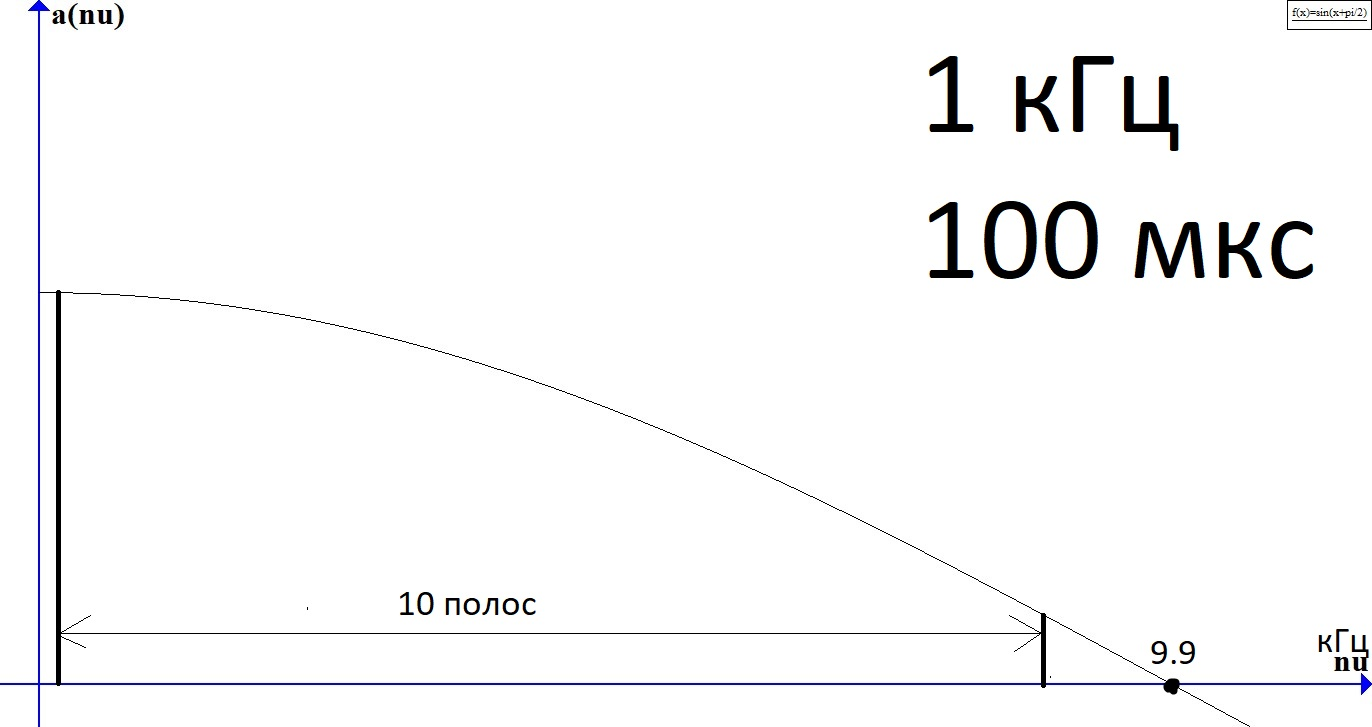
\includegraphics[scale=0.342]{1100} \\
\end{center}

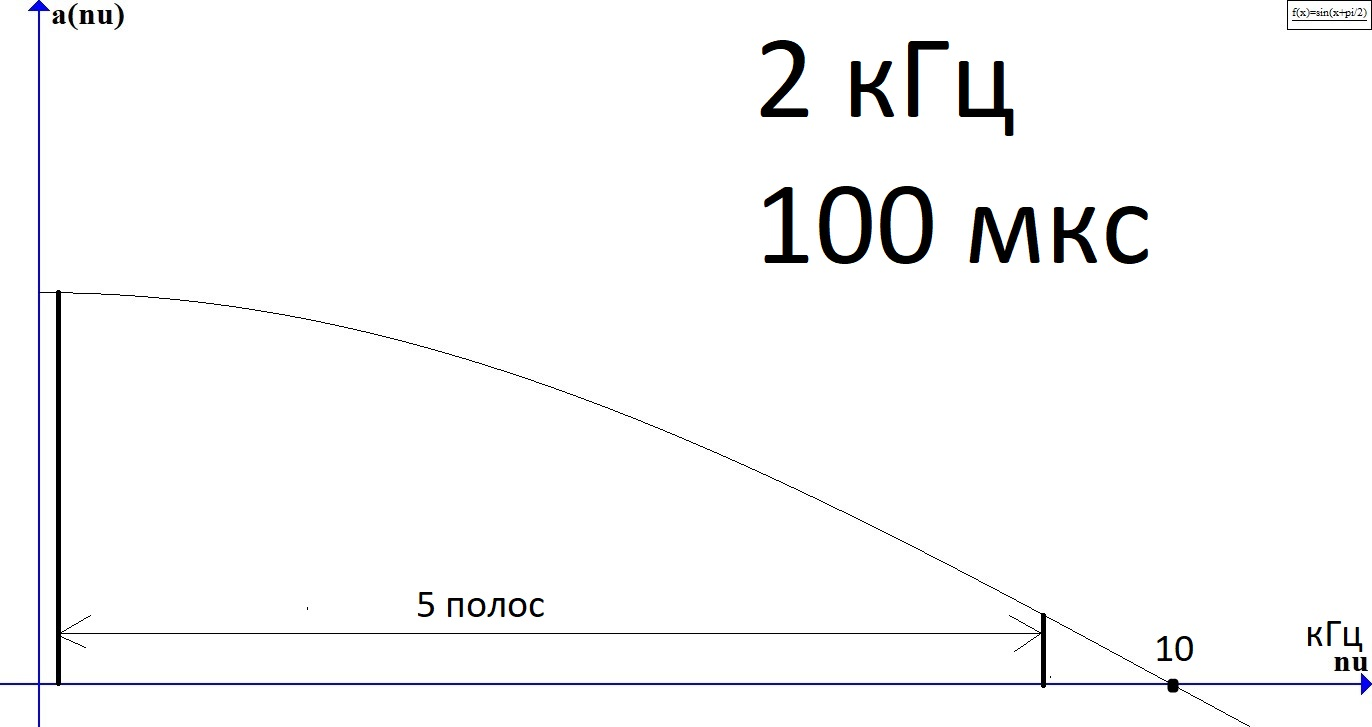
\includegraphics[scale=0.4]{2100}\\

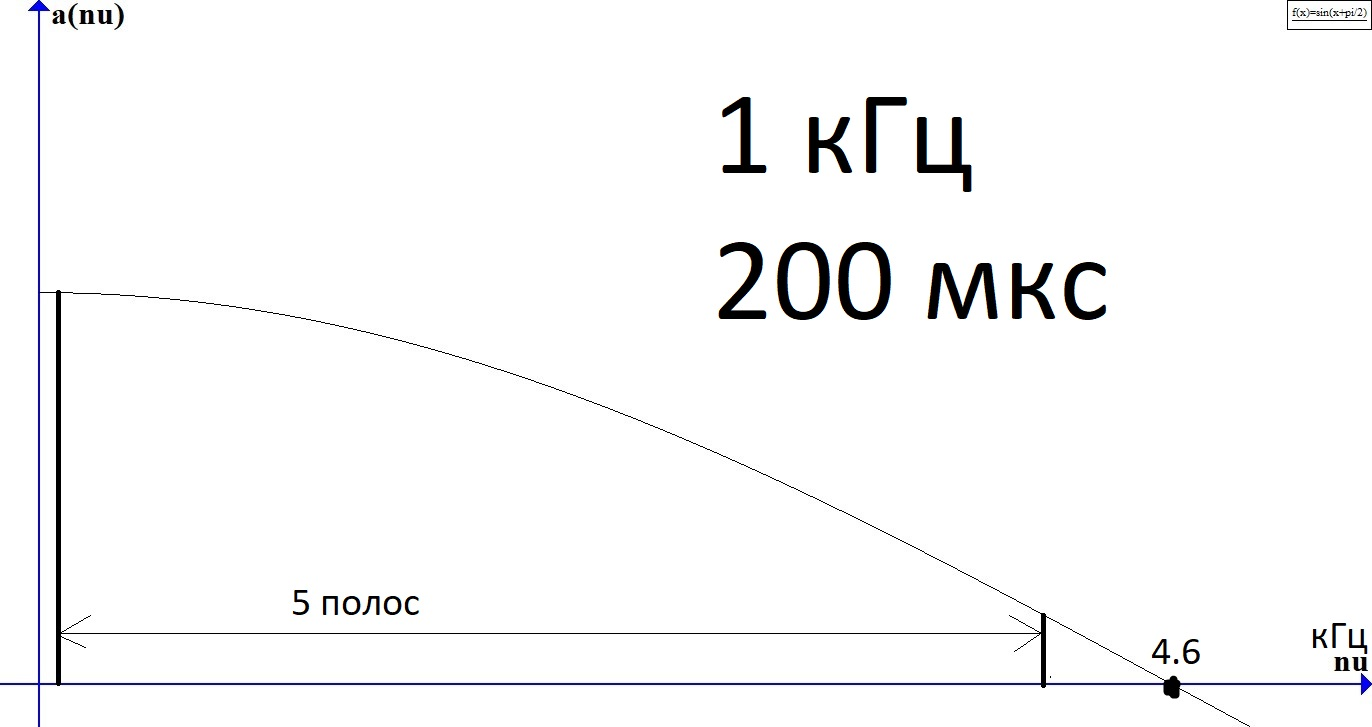
\includegraphics[scale=0.4]{1200}\\


\end{flushleft}


2) Установили $\tau$ = 50 мкс и $f_{povt}$= 1 кГц. Определим амплитуды и частоты гармоник спектра и результаты запишем в таблицу: \\
\begin{center}

\begin{tabular}{|c|c|c|}
\hline 
N & $f_{povt}$, кГц & U, mВ \\ 
\hline 
0 & 0 & 20.6 \\ 
\hline 
1 & 0.997 & 2.89 \\ 
\hline 
2 & 1.996 & 2.77 \\ 
\hline 
3 & 3.015 & 2.52 \\ 
\hline 
4 & 3.994 & 2.46 \\ 
\hline 
5 & 5 & 2.3 \\ 
\hline 
6 & 6 & 2.27 \\ 
\hline 
7 & 7 & 2.2 \\ 
\hline 
8 & 7.99 & 2.1 \\ 
\hline 
9 & 9 & 2.0 \\ 
\hline 
10 & 10.01 & 1.7 \\ 
\hline 
11 & 11 & 1.6 \\ 
\hline 
12 & 12 & 1.4 \\ 
\hline 
13 & 13 & 1.17 \\ 
\hline 
14 & 14 & 0.92 \\ 
\hline 
\end{tabular} 
\end{center}

По этим данным построим картину спектра: \\
\begin{center}

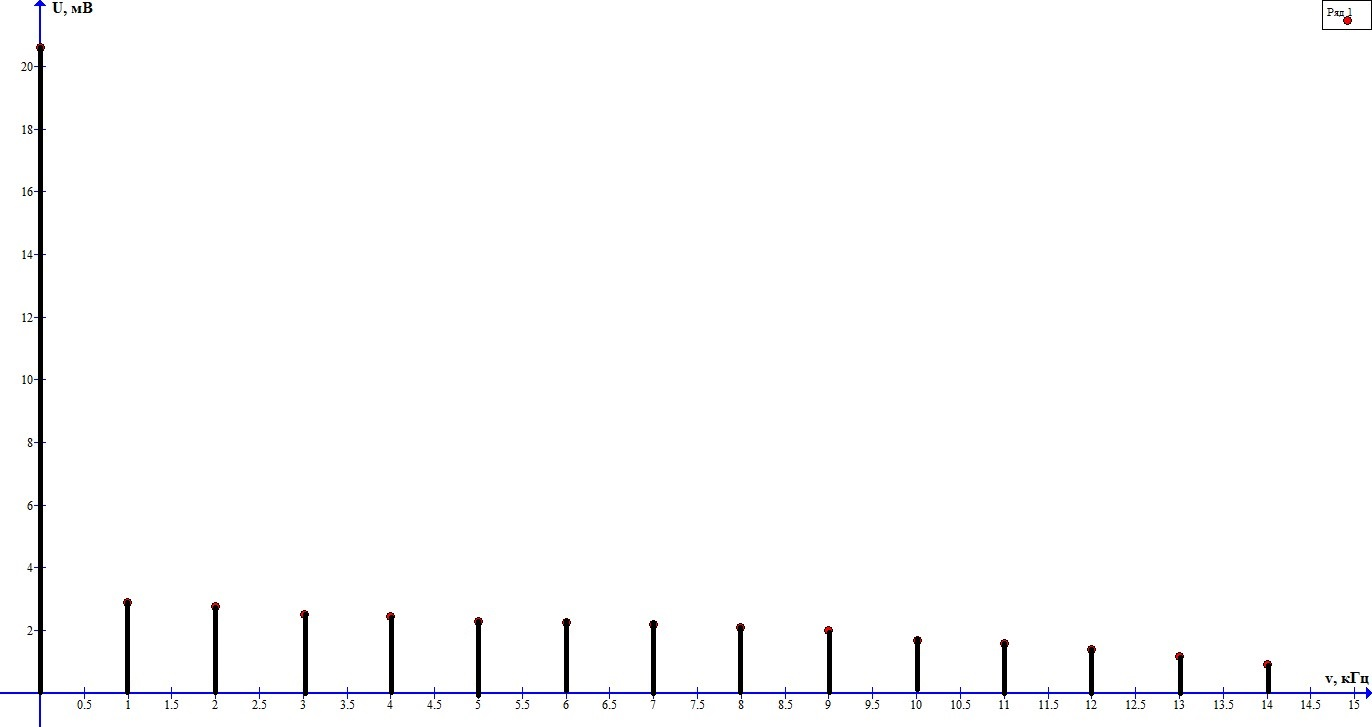
\includegraphics[scale=0.5]{312} \\
\end{center}


3) Провели измерения зависимости ширины спектра от длительности
импульса. Результаты занесли в таблицу: 
\begin{center}

	\begin{tabular}{|c|c|c|c|c|c|c|c|c|}
\hline 
$\tau$, мкс & 40 & 60 & 80 & 100 & 120 & 140 & 160 & 180 \\ 
\hline 
$\Delta\nu$, кГц & 20.5 & 15.44 & 11.79 & 9.8 & 8.6 & 7 & 5.9 & 5.3 \\ 
\hline 
1/$\tau$, мкс$^{-1}$ & 0.025 & 0.016 & 0.0125 & 0.01 & 0.008 & 0.007 & 0.006 & 0.0055 \\ 
\hline 
\end{tabular} 
\end{center}


Построим по ней график: \\
\begin{flushleft}

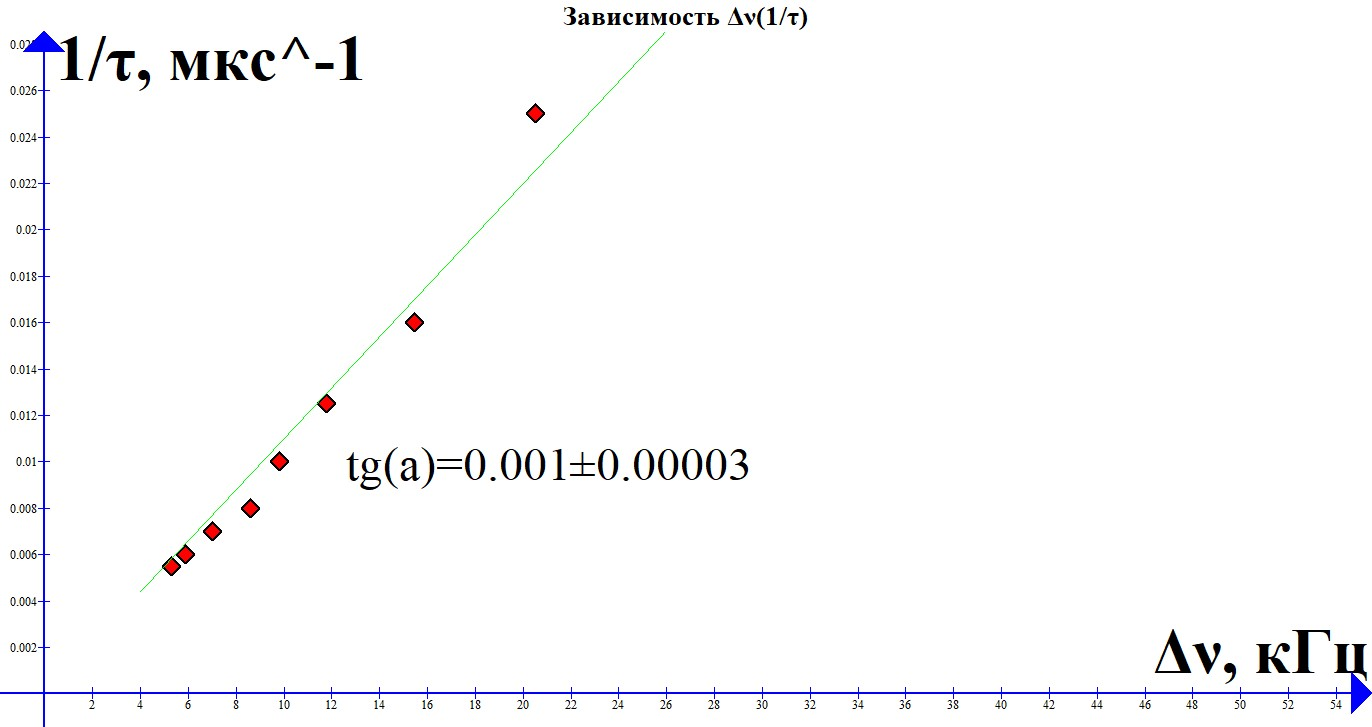
\includegraphics[scale=0.35]{3612}


\end{flushleft} 

3) Соотношение неопределенности, полученное из графика, совпадает с теоретичеким: 1000*tg(a)$\simeq$1\\
\textbf{II Исследование спектра периодической последовательности
цугов гармонических колебаний}\\
  4) Установим несущую частоту, равную 25 кГц и проследиим как меняется вид спектра при изменении длительности импульса вдвое:
\begin{flushleft}
\begin{center}

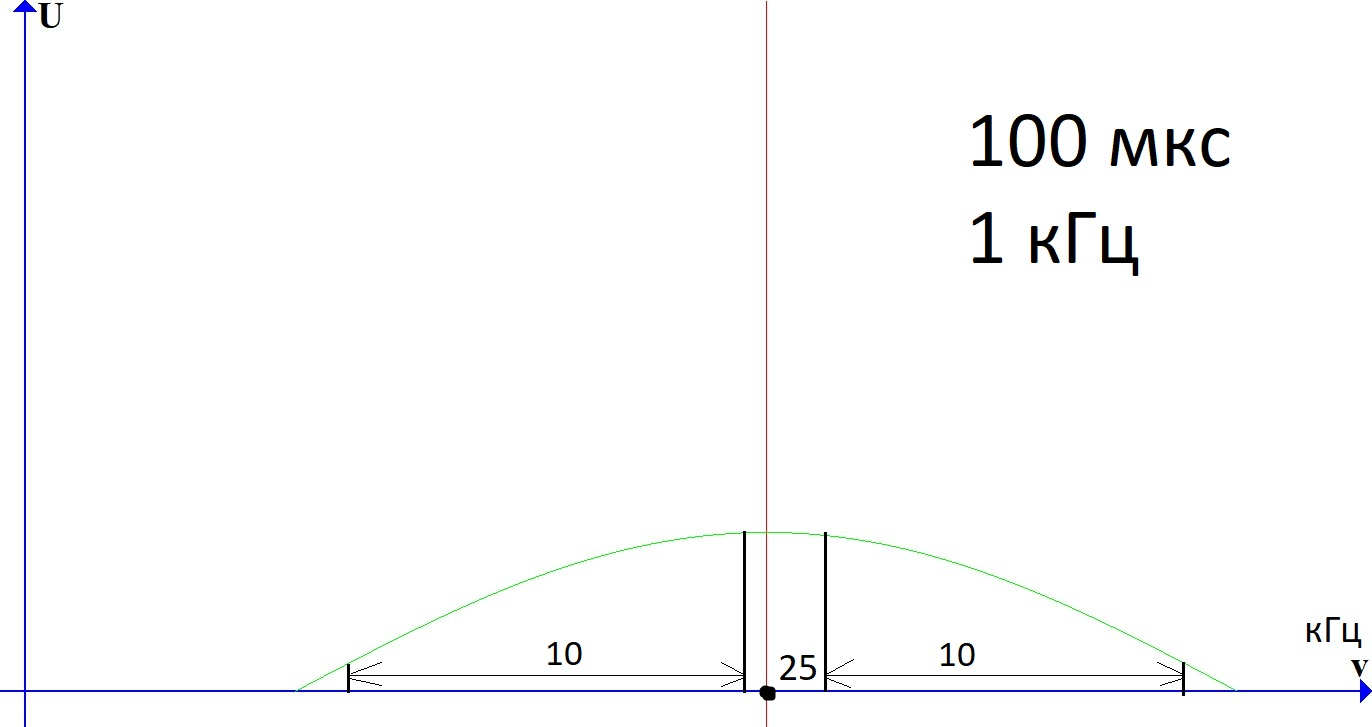
\includegraphics[scale=0.47]{1001} 
\end{center}

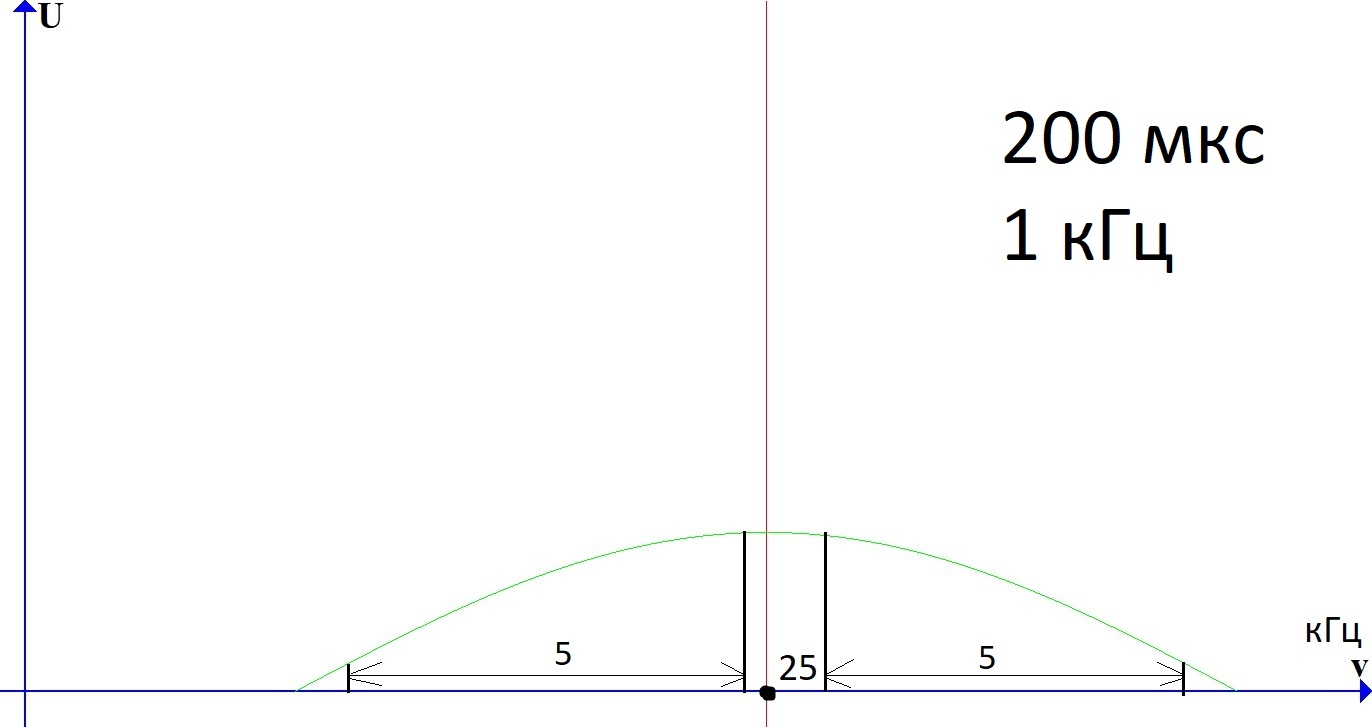
\includegraphics[scale=0.55]{2001} \\

\end{flushleft}

Из изображений видно, что число прямоугольных импульсов уменьшается, при увеличении длительности импульса\\
5) Проследим, как меняется картина
спектра при изменении несущей частоты $\nu_0$ ($\nu_0$ = 10, 25 и 40 кГц) и постоянной длительностью импульса $\tau$=100 мкс \\

\begin{flushleft}

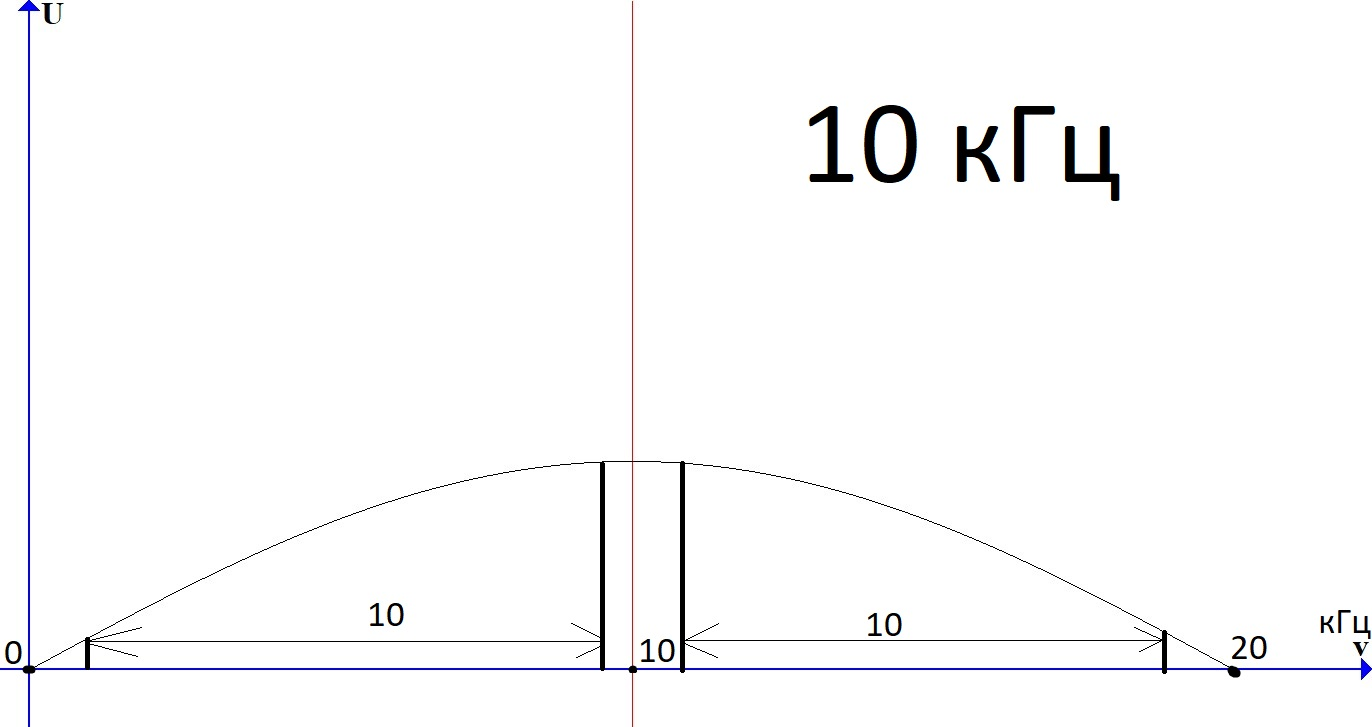
\includegraphics[scale=0.55]{10} \\
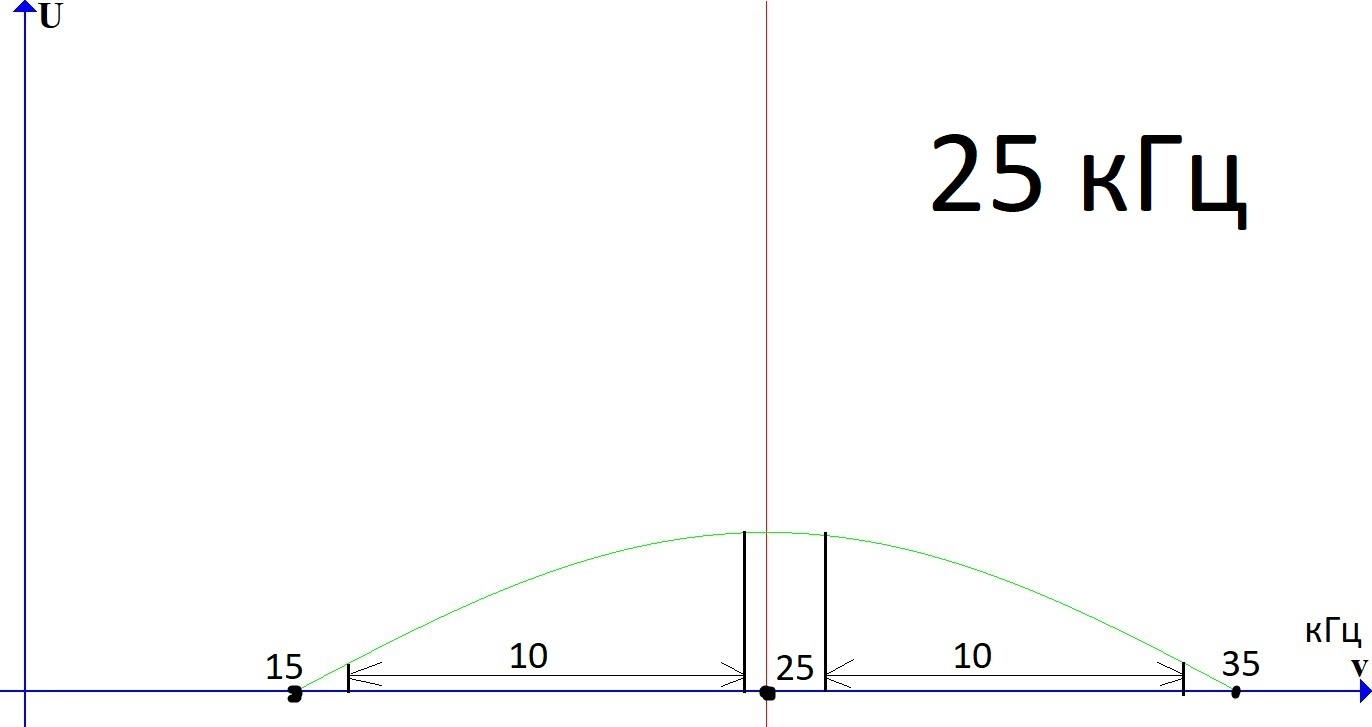
\includegraphics[scale=0.55]{25} \\
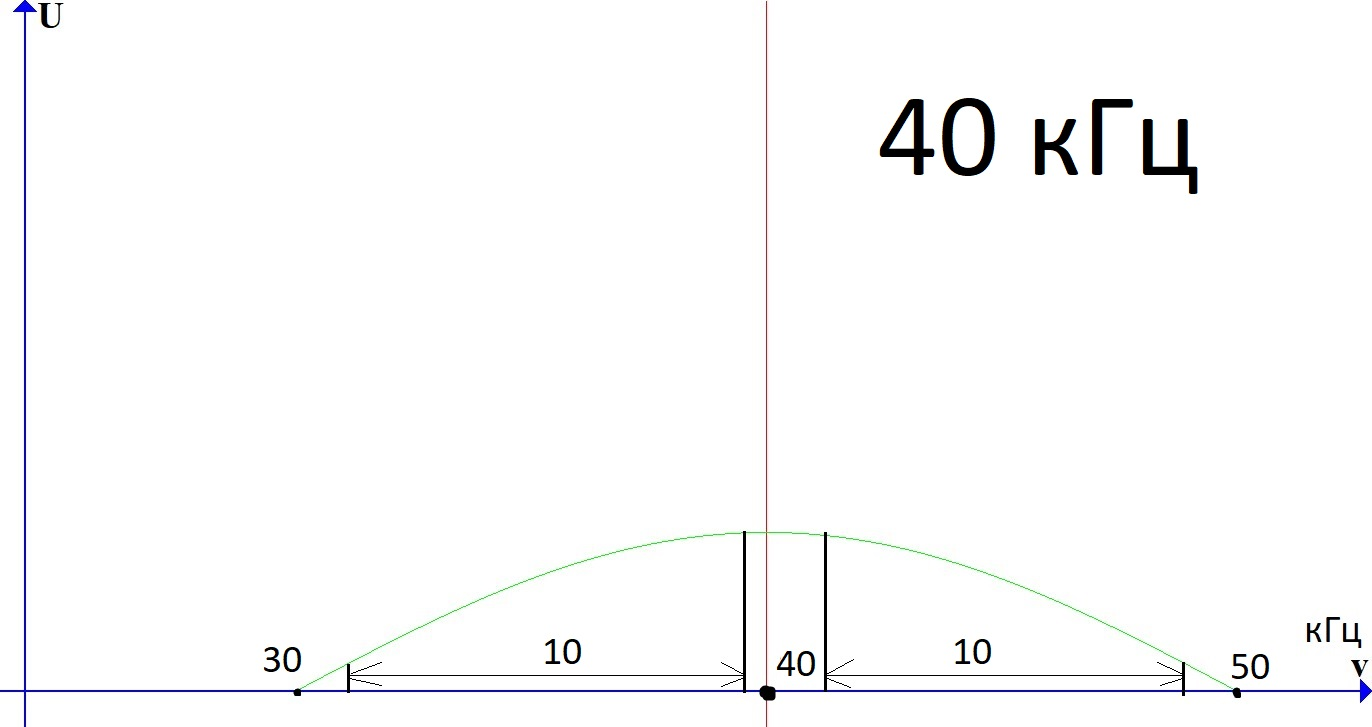
\includegraphics[scale=0.55]{40} \\

\end{flushleft}
Как видно из изображений, максимумы цугов сдвинуты по частоте на величину  $\nu_0$\\


6) Установили несущую частоту $\nu$=30 кГц, длительность импульса $\tau$ = 100
мкс. Определим расстояние $\Delta$$\nu$ между соседними спектральными компонентами
для разных частот повторения импульсов $f_{povt}$. \\
\begin{center}

\begin{tabular}{|c|c|c|c|c|c|}
\hline 
$f_{povt}$, кГц & 0.5 & 1 & 2 & 4 & 5 \\ 
\hline 
$\delta$$\nu_0$, кГц & 0.5 & 1 & 2 & 4 & 5 \\ 
\hline 
\end{tabular} 
\end{center}
Как видно из таблицы, угловой коэффицент графика зависимости $\delta$$\nu_0$($f_{povt}$) равен 1, что снова подтверждает соотношение неопределенности\\


\textbf{III Исследование спектра гармонических сигналов,
модулированных по амплитуде}\\

7) Меняя двойную амплитуду сигнала от 0,2 до 2 В измерим для каждого значения максимальную
$A_{max}$ и минимальную $A_{min}$ амплитуды сигналов модулированного колебания и амплитуды спектральных
компонент. Результаты запишем в таблицу:
\begin{center}

\begin{tabular}{|c|c|c|c|c|c|c|}
\hline 
U, В & 0.2 & 0.5 & 0.8 & 1.1 & 1.4 & 1.7 \\ 
\hline 
$2A_{max}$, В & 0.6 & 0.681 & 0.76 & 0.84 & 0.92 & 1.01 \\ 
\hline 
$2A_{min}$, В & 0.48 & 0.4 & 0.32 & 0.24 & 0.16 & 0.08 \\ 
\hline 
$a_{osn}$, В & 0.36 & 0.35 & 0.356 & 0.359 & 0.355 & 0.354 \\ 
\hline 
$a_{bok}$, В & 0.018 & 0.045 & 0.069 & 0.097 & 0.126 & 0.15 \\ 
\hline 
$a_{osn}$/$a_{bok}$ & 0.05 & 0.13 & 0.19 & 0.27 & 0.35 & 0.42 \\ 
\hline 
m & 0.1 & 0.26 & 0.4 & 0.56 & 0.7 & 0.85 \\ 
\hline 
\end{tabular} 

\end{center}


Построим по этим данным график зависимости $a_{bok}$/$a_{osn}$ от m: \\
\begin{flushleft}

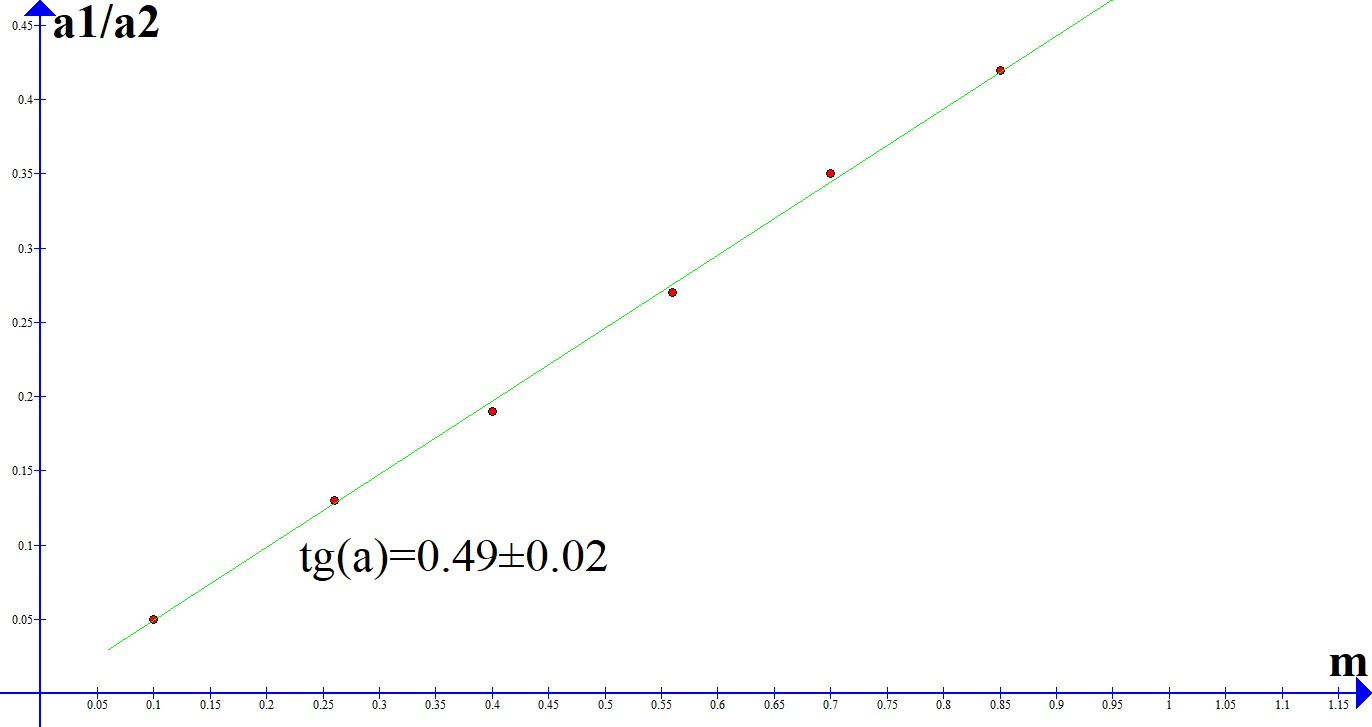
\includegraphics[scale=0.35]{5}
Коэффицент наклона практически совпадает с теоретическим значением. ($a_{osn}$=$A_0$, $a_{bok}$=$A_0$m/2, $k_{teor}$=0.5)
\\

\end{flushleft}


















\end{document} % конец документа
